% Options for packages loaded elsewhere
% Options for packages loaded elsewhere
\PassOptionsToPackage{unicode}{hyperref}
\PassOptionsToPackage{hyphens}{url}
%
\documentclass[
  ignorenonframetext,
]{beamer}
\newif\ifbibliography
\usepackage{pgfpages}
\setbeamertemplate{caption}[numbered]
\setbeamertemplate{caption label separator}{: }
\setbeamercolor{caption name}{fg=normal text.fg}
\beamertemplatenavigationsymbolsempty
% remove section numbering
\setbeamertemplate{part page}{
  \centering
  \begin{beamercolorbox}[sep=16pt,center]{part title}
    \usebeamerfont{part title}\insertpart\par
  \end{beamercolorbox}
}
\setbeamertemplate{section page}{
  \centering
  \begin{beamercolorbox}[sep=12pt,center]{section title}
    \usebeamerfont{section title}\insertsection\par
  \end{beamercolorbox}
}
\setbeamertemplate{subsection page}{
  \centering
  \begin{beamercolorbox}[sep=8pt,center]{subsection title}
    \usebeamerfont{subsection title}\insertsubsection\par
  \end{beamercolorbox}
}
% Prevent slide breaks in the middle of a paragraph
\widowpenalties 1 10000
\raggedbottom
\AtBeginPart{
  \frame{\partpage}
}
\AtBeginSection{
  \ifbibliography
  \else
    \frame{\sectionpage}
  \fi
}
\AtBeginSubsection{
  \frame{\subsectionpage}
}
\usepackage{iftex}
\ifPDFTeX
  \usepackage[T1]{fontenc}
  \usepackage[utf8]{inputenc}
  \usepackage{textcomp} % provide euro and other symbols
\else % if luatex or xetex
  \usepackage{unicode-math} % this also loads fontspec
  \defaultfontfeatures{Scale=MatchLowercase}
  \defaultfontfeatures[\rmfamily]{Ligatures=TeX,Scale=1}
\fi
\usepackage{lmodern}

\usetheme[]{CambridgeUS}
\usecolortheme[]{default}
\ifPDFTeX\else
  % xetex/luatex font selection
\fi
% Use upquote if available, for straight quotes in verbatim environments
\IfFileExists{upquote.sty}{\usepackage{upquote}}{}
\IfFileExists{microtype.sty}{% use microtype if available
  \usepackage[]{microtype}
  \UseMicrotypeSet[protrusion]{basicmath} % disable protrusion for tt fonts
}{}
\makeatletter
\@ifundefined{KOMAClassName}{% if non-KOMA class
  \IfFileExists{parskip.sty}{%
    \usepackage{parskip}
  }{% else
    \setlength{\parindent}{0pt}
    \setlength{\parskip}{6pt plus 2pt minus 1pt}}
}{% if KOMA class
  \KOMAoptions{parskip=half}}
\makeatother


\usepackage{longtable,booktabs,array}
\usepackage{calc} % for calculating minipage widths
\usepackage{caption}
% Make caption package work with longtable
\makeatletter
\def\fnum@table{\tablename~\thetable}
\makeatother
\usepackage{graphicx}
\makeatletter
\newsavebox\pandoc@box
\newcommand*\pandocbounded[1]{% scales image to fit in text height/width
  \sbox\pandoc@box{#1}%
  \Gscale@div\@tempa{\textheight}{\dimexpr\ht\pandoc@box+\dp\pandoc@box\relax}%
  \Gscale@div\@tempb{\linewidth}{\wd\pandoc@box}%
  \ifdim\@tempb\p@<\@tempa\p@\let\@tempa\@tempb\fi% select the smaller of both
  \ifdim\@tempa\p@<\p@\scalebox{\@tempa}{\usebox\pandoc@box}%
  \else\usebox{\pandoc@box}%
  \fi%
}
% Set default figure placement to htbp
\def\fps@figure{htbp}
\makeatother





\setlength{\emergencystretch}{3em} % prevent overfull lines

\providecommand{\tightlist}{%
  \setlength{\itemsep}{0pt}\setlength{\parskip}{0pt}}



 


\usepackage{amsmath}
\usepackage{amssymb}
\date{\text{Jan - May, 2026}}
\let\olddate\date
\renewcommand{\date}[1]{}
\title[SIMA]{ Statistical Inference and Multivariate Analysis (MA324) }
\subtitle{ \textsc{Lecture Slides} \\ Topic 01 \\ Delta Method and Bootstrap }
\makeatletter
\@ifpackageloaded{caption}{}{\usepackage{caption}}
\AtBeginDocument{%
\ifdefined\contentsname
  \renewcommand*\contentsname{Table of contents}
\else
  \newcommand\contentsname{Table of contents}
\fi
\ifdefined\listfigurename
  \renewcommand*\listfigurename{List of Figures}
\else
  \newcommand\listfigurename{List of Figures}
\fi
\ifdefined\listtablename
  \renewcommand*\listtablename{List of Tables}
\else
  \newcommand\listtablename{List of Tables}
\fi
\ifdefined\figurename
  \renewcommand*\figurename{Figure}
\else
  \newcommand\figurename{Figure}
\fi
\ifdefined\tablename
  \renewcommand*\tablename{Table}
\else
  \newcommand\tablename{Table}
\fi
}
\@ifpackageloaded{float}{}{\usepackage{float}}
\floatstyle{ruled}
\@ifundefined{c@chapter}{\newfloat{codelisting}{h}{lop}}{\newfloat{codelisting}{h}{lop}[chapter]}
\floatname{codelisting}{Listing}
\newcommand*\listoflistings{\listof{codelisting}{List of Listings}}
\makeatother
\makeatletter
\makeatother
\makeatletter
\@ifpackageloaded{caption}{}{\usepackage{caption}}
\@ifpackageloaded{subcaption}{}{\usepackage{subcaption}}
\makeatother

\usepackage{bookmark}
\IfFileExists{xurl.sty}{\usepackage{xurl}}{} % add URL line breaks if available
\urlstyle{same}
\hypersetup{
  hidelinks,
  pdfcreator={LaTeX via pandoc}}


\author{}
\date{}

\begin{document}


\begin{frame}[plain]{}
\phantomsection\label{section}
\titlepage
\end{frame}

\section{Delta Method}\label{delta-method}

\begin{frame}{Introduction \& Intuition}
\phantomsection\label{introduction-intuition}
\begin{itemize}
\tightlist
\item
  \textbf{The Problem:} We know the asymptotic distribution of an
  estimator \(\hat{\theta}\), but we want to know the asymptotic
  distribution of a continuous function \(g(\hat{\theta})\).
\item
  \textbf{The Solution:} The Delta Method uses a first-order Taylor
  series expansion to approximate the variance of the transformed
  estimator.
\item
  \textbf{Taylor Expansion:} Around the true parameter \(\theta\), the
  function \(g(\hat{\theta})\) can be approximated as:
  \[g(\hat{\theta}) \approx g(\theta) + g'(\theta)(\hat{\theta} - \theta)\]
\item
  Rearranging terms, we get:
  \[g(\hat{\theta}) - g(\theta) \approx g'(\theta)(\hat{\theta} - \theta)\]
\end{itemize}
\end{frame}

\begin{frame}{The Univariate Delta Method}
\phantomsection\label{the-univariate-delta-method}
Let \(X_n\) be a sequence of random variables such that:
\[\sqrt{n}(X_n - \theta) \xrightarrow{d} \mathcal{N}(0, \sigma^2)\]
Suppose \(g\) is a function such that its derivative \(g'(\theta)\)
exists and is non-zero. Then:
\[\sqrt{n}(g(X_n) - g(\theta)) \xrightarrow{d} \mathcal{N}\left(0, \sigma^2 \left[g'(\theta)\right]^2\right)\]

\vspace{0.5cm}

\textbf{Implication:} The variance of the transformed estimator is
approximately the original variance multiplied by the square of the
derivative of the transformation evaluated at \(\theta\).
\end{frame}

\begin{frame}{Proof Sketch: Univariate Delta Method}
\phantomsection\label{proof-sketch-univariate-delta-method}
\begin{itemize}
\tightlist
\item
  By Taylor's Theorem and the Mean Value Theorem, we can write:
  \[g(X_n) = g(\theta) + g'(\tilde{\theta})(X_n - \theta)\] where
  \(\tilde{\theta}\) lies strictly between \(X_n\) and \(\theta\).
\item
  Rearranging and multiplying by \(\sqrt{n}\):
  \[\sqrt{n}(g(X_n) - g(\theta)) = g'(\tilde{\theta})\sqrt{n}(X_n - \theta)\]
\item
  Since
  \(\sqrt{n}(X_n - \theta) \xrightarrow{d} \mathcal{N}(0, \sigma^2)\),
  we know \(X_n \xrightarrow{p} \theta\). Thus,
  \(\tilde{\theta} \xrightarrow{p} \theta\).
\item
  By the Continuous Mapping Theorem,
  \(g'(\tilde{\theta}) \xrightarrow{p} g'(\theta)\).
\item
  Finally, applying \textbf{Slutsky's Theorem}:
  \[g'(\tilde{\theta})\sqrt{n}(X_n - \theta) \xrightarrow{d} g'(\theta) \cdot \mathcal{N}(0, \sigma^2) \equiv \mathcal{N}\left(0, \sigma^2 [g'(\theta)]^2\right)\]
\end{itemize}
\end{frame}

\begin{frame}{Example: Estimating Survival Probability}
\phantomsection\label{example-estimating-survival-probability}
\begin{itemize}
\tightlist
\item
  Let lifetimes \(T_1, \dots, T_n \sim \text{Exp}(\lambda)\). The MLE
  for the rate is \(\hat{\lambda} = 1/\bar{T}\).
\item
  From asymptotic likelihood theory, we know:
  \[\sqrt{n}(\hat{\lambda} - \lambda) \xrightarrow{d} \mathcal{N}(0, \lambda^2)\]
\item
  We want the asymptotic distribution of the survival function at time
  \(t_0\): \(S(t_0) = \exp(-\lambda t_0)\).
\item
  Let \(g(\lambda) = \exp(-\lambda t_0)\). The derivative is
  \(g'(\lambda) = -t_0 \exp(-\lambda t_0)\).
\item
  Applying the Delta Method:
  \[\sqrt{n}\left(\exp(-\hat{\lambda} t_0) - \exp(-\lambda t_0)\right) \xrightarrow{d} \mathcal{N}\left(0, \lambda^2 \left[-t_0 \exp(-\lambda t_0)\right]^2\right)\]
\item
  The asymptotic variance simplifies to
  \(\lambda^2 t_0^2 \exp(-2\lambda t_0)\).
\end{itemize}
\end{frame}

\begin{frame}{Constructing Confidence Intervals}
\phantomsection\label{constructing-confidence-intervals}
\begin{itemize}
\tightlist
\item
  We use a plug-in estimator for the standard error. Let
  \(\widehat{\text{SE}}(g(\hat{\theta}))\) be:
  \[\widehat{\text{SE}}(g(\hat{\theta})) = \sqrt{\frac{\hat{\sigma}^2 \left[g'(\hat{\theta})\right]^2}{n}}\]
\item
  An approximate \((1 - \alpha)100\%\) confidence interval for
  \(g(\theta)\) is:
  \[g(\hat{\theta}) \pm z_{\alpha/2} \cdot \widehat{\text{SE}}(g(\hat{\theta}))\]
\item
  Returning to our survival example,
  \(\hat{S}(t_0) = \exp(-\hat{\lambda} t_0)\).
\item
  The estimated standard error is:
  \[\widehat{\text{SE}}(\hat{S}(t_0)) = \frac{\hat{\lambda} t_0 \exp(-\hat{\lambda} t_0)}{\sqrt{n}}\]
\item
  A \((1 - \alpha)100\%\) asymptotic CI for \(S(t_0)\) is:
  \[\exp(-\hat{\lambda} t_0) \pm z_{\alpha/2} \left[ \frac{\hat{\lambda} t_0 \exp(-\hat{\lambda} t_0)}{\sqrt{n}} \right]\]
\end{itemize}
\end{frame}

\begin{frame}{Restricting Survival CIs to \([0, 1]\)}
\phantomsection\label{restricting-survival-cis-to-0-1}
\begin{itemize}
\tightlist
\item
  The standard linear CI for \(\hat{S}(t_0)\) can yield bounds outside
  \([0, 1]\).
\item
  \textbf{Solution:} Apply the Delta Method to a transformation that
  maps \((0, 1)\) to \((-\infty, \infty)\), such as the complementary
  log-log transformation: \(g(S) = \ln(-\ln(S))\).
\item
  The derivative is \(g'(S) = \frac{1}{S \ln(S)}\). By the Delta Method:
  \[\widehat{\text{Var}}(\ln(-\ln(\hat{S}))) \approx \left[ \frac{1}{\hat{S} \ln(\hat{S})} \right]^2 \widehat{\text{Var}}(\hat{S})\]
\item
  Calculate the CI bounds for the transformed parameter:
  \[[L_W, U_W] = \ln(-\ln(\hat{S})) \pm z_{\alpha/2} \cdot \widehat{\text{SE}}(\ln(-\ln(\hat{S})))\]
\item
  Transform back to get the \([0, 1]\)-restricted CI for \(S(t_0)\):
  \[\left[ \exp(-\exp(U_W)), \exp(-\exp(L_W)) \right]\]
\end{itemize}
\end{frame}

\begin{frame}{Simulation: Linear vs.~Log-Log Bounds}
\phantomsection\label{simulation-linear-vs.-log-log-bounds}
\begin{center}
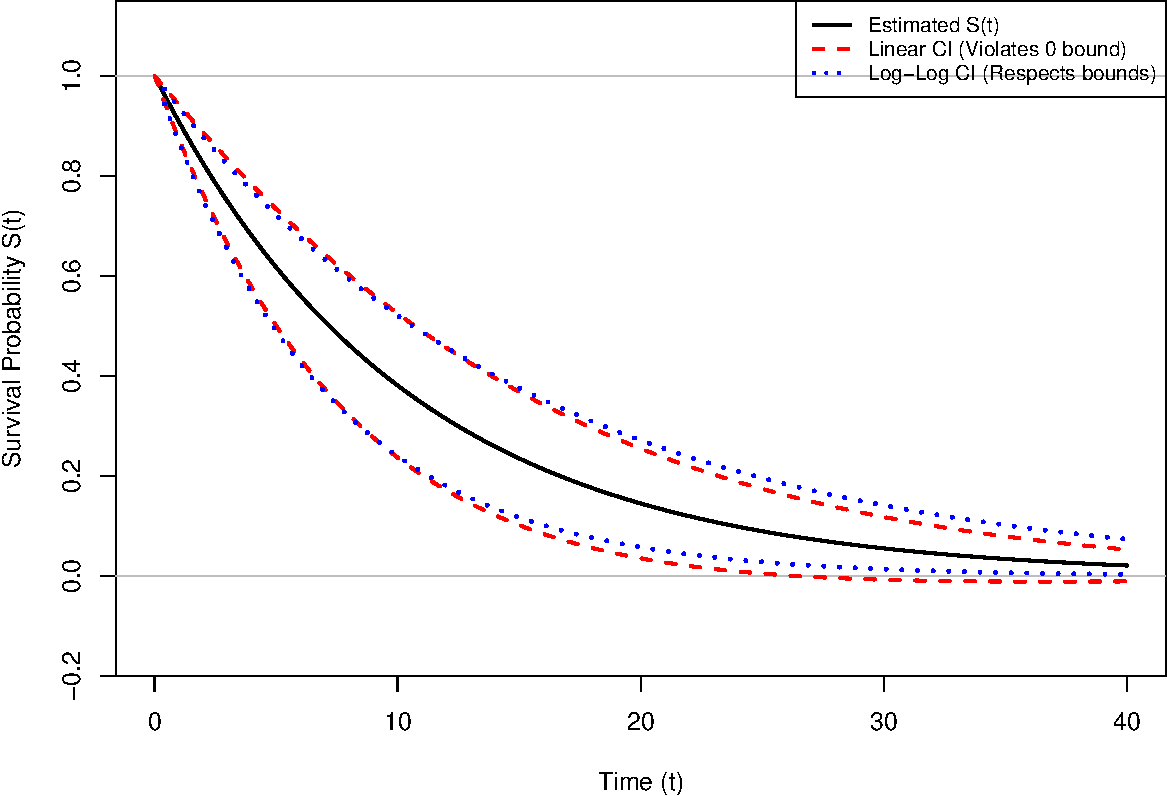
\includegraphics[width=0.9\linewidth,height=\textheight,keepaspectratio]{topic01-CI_files/figure-beamer/survival-ci-plot-1.pdf}
\end{center}
\end{frame}

\begin{frame}{The Second-Order Delta Method}
\phantomsection\label{the-second-order-delta-method}
\begin{itemize}
\tightlist
\item
  \textbf{Question:} What happens if \(g'(\theta) = 0\)? The first-order
  approximation collapses to \(0\).
\item
  If \(g'(\theta) = 0\) but \(g''(\theta) \neq 0\), we extend the Taylor
  series to the second order:
  \[g(X_n) \approx g(\theta) + g'(\theta)(X_n - \theta) + \frac{1}{2}g''(\theta)(X_n - \theta)^2\]
\item
  Since \(g'(\theta) = 0\), we multiply both sides by \(n\) (instead of
  \(\sqrt{n}\)):
  \[n(g(X_n) - g(\theta)) \approx \frac{1}{2}g''(\theta) \left[\sqrt{n}(X_n - \theta)\right]^2\]
\item
  Because
  \(\sqrt{n}(X_n - \theta) \xrightarrow{d} \mathcal{N}(0, \sigma^2)\),
  its square converges to \(\sigma^2 \chi^2_1\).
\item
  \textbf{Result:}
  \(n(g(X_n) - g(\theta)) \xrightarrow{d} \frac{1}{2} \sigma^2 g''(\theta) \chi^2_1\).
\end{itemize}
\end{frame}

\begin{frame}{The Multivariate Delta Method}
\phantomsection\label{the-multivariate-delta-method}
\begin{block}{Theorem}
Let $\mathbf{X}_n$ be a sequence of random vectors in $\mathbb{R}^k$ such that:
$$\sqrt{n}(\mathbf{X}_n - \boldsymbol{\theta}) \xrightarrow{d} \mathcal{N}_k(\mathbf{0}, \Sigma)$$
Let $g: \mathbb{R}^k \rightarrow \mathbb{R}^m$ be a function whose Jacobian matrix $\nabla g(\boldsymbol{\theta})$ (of size $m \times k$) is evaluated at $\boldsymbol{\theta}$. Then:
$$\sqrt{n}(g(\mathbf{X}_n) - g(\boldsymbol{\theta})) \xrightarrow{d} \mathcal{N}_m\left(\mathbf{0}, \nabla g(\boldsymbol{\theta}) \Sigma \nabla g(\boldsymbol{\theta})^T\right)$$
\end{block}

\vspace{0.2cm}

\emph{Note: The matrix
\(\nabla g(\boldsymbol{\theta}) \Sigma \nabla g(\boldsymbol{\theta})^T\)
is the asymptotic covariance matrix of the transformed vector.}
\end{frame}

\section{Bootstrap}\label{bootstrap}

\begin{frame}{Bootstrap}
\phantomsection\label{bootstrap-1}
\begin{itemize}
\tightlist
\item
  A {widely applicable and extremely powerful} statistical tool.
\item
  It can be used to {quantify the uncertainty associated with a given
  estimator} or statistical learning method.
\item
  As a simple example, the bootstrap can be used {to estimate the
  standard errors of the coefficients} from a \textbf{linear regression}
  fit.
\item
  In the specific {case of linear regression, this is not particularly
  useful}, since standard statistical software such as R outputs such
  standard errors automatically.
\item
  The power of the bootstrap lies in the fact that it can be easily
  applied to {a wide range of statistical learning methods:}

  \begin{itemize}
  \tightlist
  \item
    including some for which {a measure of variability is otherwise
    difficult to obtain} and is not automatically output by statistical
    software.
  \end{itemize}
\end{itemize}
\end{frame}

\begin{frame}{A toy example:}
\phantomsection\label{a-toy-example}
\begin{itemize}
\tightlist
\item
  Let Singapore Govt. wants to {invest an extra fixed sum of money in
  two health systems (hospital or polyclinics)} that yield returns of
  \(X\) and \(Y\), respectively, where \(X\) and \(Y\) are random
  quantities.
\item
  Govt. will invest a {fraction \(\alpha\) of it's money in \(X\)}, and
  will invest the {remaining \(1 - \alpha\) in \(Y\).}
\item
  Since there is variability associated with the returns on these two
  systems, Govt. wants to {choose \(\alpha\) to minimize the total risk,
  or variance,} of the investment.
\item
  In other words, Govt. wants to minimize
  \(Var(\alpha X + (1 -\alpha)Y )\).
\item
  One can show that the value that minimizes the risk is given by
  \[\alpha = \frac{\sigma_{Y}^2 - \sigma_{XY}}{\sigma_{X}^2 + \sigma_{Y}^2 - 2\sigma_{XY}},\]
  where \(\sigma_{X}^2 = var(X)\), \(\sigma_{Y}^2 = var(Y)\) and
  \(\sigma_{XY} = cov(X, Y)\).
\end{itemize}
\end{frame}

\begin{frame}{A toy example: (cont.)}
\phantomsection\label{a-toy-example-cont.}
\begin{itemize}
\tightlist
\item
  In practice, \(\sigma_{X}^2, \sigma_{Y}^2\) and \(\sigma_{XY}\) are
  unknown.
\item
  Let from past real data (on \(X\) and \(Y\)), we can get the estimates
  of the above as \(\hat\sigma_{X}^2, \hat\sigma_{Y}^2\) and
  \(\hat\sigma_{XY}\).
\item
  We can then estimate the value of \(\alpha\) that minimizes the
  variance of Govt. investment using
  \[\hat\alpha = \frac{\hat\sigma_{Y}^2 - \hat\sigma_{XY}}{\hat\sigma_{X}^2 + \hat\sigma_{Y}^2 - 2\hat\sigma_{XY}}.\]
\item
  How do you find a variance (accuracy of the estimate) of
  \(\hat \alpha\)?
\end{itemize}
\end{frame}

\begin{frame}{A toy example: variance}
\phantomsection\label{a-toy-example-variance}
\begin{itemize}
\tightlist
\item
  To estimate the standard deviation of \(\hat \alpha\) we need to (some
  how) know the distribution of \(\hat \alpha\).
\item
  Let there are 100 pairs of observation on \((X, Y)\).
\item
  Let generate one random sample (with replacement) of size 100 from the
  above real data.
\item
  Now repeat the the above process (sample generation) for 1000 times.
\item
  Then we have 1,000 estimates for \(\alpha\) each from one sample,
  which we can call
  \[\hat\alpha_1, \hat\alpha_2, \cdots, \hat\alpha_{1000}.\]
\end{itemize}
\end{frame}

\begin{frame}{A toy example: (cont.)}
\phantomsection\label{a-toy-example-cont.-1}
\begin{itemize}
\tightlist
\item
  The Bootstrap estimate of \(\alpha\) based on 1000 samples is:
  \[\bar{\alpha} = \frac{1}{1000} \sum_{r=1}^{1000} \hat{\alpha}_r\]
\item
  The Bootstrap estimate of the variance of \(\hat\alpha\) based on 1000
  samples is:
  \[\frac{1}{1000-1} \sum_{r=1}^{1000}(\hat{\alpha}_r - \bar{\alpha})^2.\]
\end{itemize}
\end{frame}

\begin{frame}{Non-Parametric Bootstrap:}
\phantomsection\label{non-parametric-bootstrap}
\begin{itemize}
\tightlist
\item
  Consider a {data of size \(n\)} as: \(x_1, \cdots, x_n\).
\item
  We want to find the {bootstrap estimate of variance of the estimator
  \(T(X)\)}
\item
  {Randomly select \(n\) observations} from the data set in order to
  produce a bootstrap data set, \(Z^{*1}\).
\item
  The {sampling is performed with replacement,} which means that the
  same observation can occur more than once in the bootstrap data set.
\item
  We can use \(Z^{*1}\) to {produce a new bootstrap estimate} for
  \(T(X)\), which we call \(T_1^*(x)\).
\end{itemize}
\end{frame}

\begin{frame}{Non-Parametric Bootstrap: (cont.)}
\phantomsection\label{non-parametric-bootstrap-cont.}
\begin{itemize}
\tightlist
\item
  This procedure is {repeated \(B\) times} for some large value of
  \(B\), in order to produce \(B\) {different bootstrap data sets,}
  \(Z^{*1}, Z^{*2}, \cdots, Z^{*B}\), and
\item
  \(B\) (corresponding \(T(X)\)) estimates as
  \(T_1^*(x), T_2^*(x), \cdots, T_B^*(x)\).
\item
  We can compute the {variance of these bootstrap estimates} using the
  formula
  \[var(\hat T(X)) = \frac{1}{B-1} \sum_{r=1}^{B} \bigg(T_r^*(x) - \frac{1}{B}\sum_{r'=1}^{B} T_{r'}^*(x) \bigg)^2\]
\item
  This serves as an estimate of the variance of \(\hat T(X)\), estimated
  from the original data set.
\end{itemize}
\end{frame}

\begin{frame}{Parametric Bootstrap:}
\phantomsection\label{parametric-bootstrap}
\begin{itemize}
\tightlist
\item
  Let \(x_1, \cdots, x_n\) are {obtained independently from
  \(N(\mu, 1)\).}
\item
  Estimate \(\mu\) (using MLE) as: \(\hat \mu = \bar{x}\).
\item
  Generate a {sample of size \(n\) from \(N(\bar{x}, 1)\)} and estimate
  the sample mean as \(\bar{x}_1\) from this newly generate samples.
\item
  {Repeat the above \(B\) times to get \(B\) such estimates} as
  \(\bar{x}_1, \cdots, \bar{x}_B\).
\item
  The {variance of \(\bar{x}\) based on the bootstrap} estimates
  \[var(\bar{x}) = \frac{1}{B-1} \sum_{r=1}^{B} \bigg(\bar{x}_r - \frac{1}{B}\sum_{r'=1}^{B} \bar{x}_{r'} \bigg)^2.\]
\end{itemize}
\end{frame}

\begin{frame}{An empirical bootstrap confidence interval:}
\phantomsection\label{an-empirical-bootstrap-confidence-interval}
\begin{itemize}
\tightlist
\item
  The {sample data:} 30, 37, 36, 43, 42, 43, 43, 46, 41, 42
\item
  Problem: {Estimate the mean \(\mu\)} of the underlying distribution
  and give an {80\% bootstrap confidence interval.}
\item
  The sample mean is \(\bar{x} = 40.3\). We {use this as an estimate} of
  the true mean \(\mu\) of the underlying distribution.
\item
  To make the confidence interval we need to know how much the
  {distribution of \(\bar{x}\) varies around \(\mu\).}
\item
  In fact, we want to know the {distribution of
  \(\delta = \bar{x} - \mu\)}.
\end{itemize}
\end{frame}

\begin{frame}{An empirical bootstrap confidence interval: (cont.)}
\phantomsection\label{an-empirical-bootstrap-confidence-interval-cont.}
\begin{itemize}
\tightlist
\item
  If we {knew this distribution} we could find \(\delta_{0.1}\) and
  \(\delta_{0.9}\), the 0.1 and 0.9 critical values of \(\delta\).
\item
  Then we would have
  \[P(\delta_{0.9} \leq \bar{x} - \mu \leq \delta_{0.1} | \mu) = 0.8 \implies P(\bar{x} - \delta_{0.9} \geq \mu \geq \bar{x} - \delta_{0.1} | \mu ) = 0.8\]
  which gives {an 80\% confidence interval} of
  \([\bar{x} - \delta_{0.1}, \bar{x} - \delta_{0.9} ]\).
\item
  The bootstrap principle offers a {practical approach to estimating the
  distribution} of \(\delta = \bar{x} - \mu\).
\item
  It says that we can approximate it by the distribution of
  \(\delta^* = \bar{x}^* - \bar{x}\) where \(\bar{x}^*\) is the mean of
  an empirical bootstrap sample.
\end{itemize}
\end{frame}

\begin{frame}{An empirical bootstrap confidence interval: (cont.)}
\phantomsection\label{an-empirical-bootstrap-confidence-interval-cont.-1}
\textbf{Bootstrap Samples (20 iterations):}

\begin{longtable}[]{@{}
  >{\raggedright\arraybackslash}p{(\linewidth - 38\tabcolsep) * \real{0.0500}}
  >{\raggedright\arraybackslash}p{(\linewidth - 38\tabcolsep) * \real{0.0500}}
  >{\raggedright\arraybackslash}p{(\linewidth - 38\tabcolsep) * \real{0.0500}}
  >{\raggedright\arraybackslash}p{(\linewidth - 38\tabcolsep) * \real{0.0500}}
  >{\raggedright\arraybackslash}p{(\linewidth - 38\tabcolsep) * \real{0.0500}}
  >{\raggedright\arraybackslash}p{(\linewidth - 38\tabcolsep) * \real{0.0500}}
  >{\raggedright\arraybackslash}p{(\linewidth - 38\tabcolsep) * \real{0.0500}}
  >{\raggedright\arraybackslash}p{(\linewidth - 38\tabcolsep) * \real{0.0500}}
  >{\raggedright\arraybackslash}p{(\linewidth - 38\tabcolsep) * \real{0.0500}}
  >{\raggedright\arraybackslash}p{(\linewidth - 38\tabcolsep) * \real{0.0500}}
  >{\raggedright\arraybackslash}p{(\linewidth - 38\tabcolsep) * \real{0.0500}}
  >{\raggedright\arraybackslash}p{(\linewidth - 38\tabcolsep) * \real{0.0500}}
  >{\raggedright\arraybackslash}p{(\linewidth - 38\tabcolsep) * \real{0.0500}}
  >{\raggedright\arraybackslash}p{(\linewidth - 38\tabcolsep) * \real{0.0500}}
  >{\raggedright\arraybackslash}p{(\linewidth - 38\tabcolsep) * \real{0.0500}}
  >{\raggedright\arraybackslash}p{(\linewidth - 38\tabcolsep) * \real{0.0500}}
  >{\raggedright\arraybackslash}p{(\linewidth - 38\tabcolsep) * \real{0.0500}}
  >{\raggedright\arraybackslash}p{(\linewidth - 38\tabcolsep) * \real{0.0500}}
  >{\raggedright\arraybackslash}p{(\linewidth - 38\tabcolsep) * \real{0.0500}}
  >{\raggedright\arraybackslash}p{(\linewidth - 38\tabcolsep) * \real{0.0500}}@{}}
\toprule\noalign{}
\endhead
43 & 36 & 46 & 30 & 43 & 43 & 43 & 37 & 42 & 42 & 43 & 37 & 36 & 42 & 43
& 43 & 42 & 43 & 42 & 43 \\
43 & 41 & 37 & 37 & 43 & 43 & 46 & 36 & 41 & 43 & 43 & 42 & 41 & 43 & 46
& 36 & 43 & 43 & 43 & 42 \\
42 & 43 & 37 & 43 & 46 & 37 & 36 & 41 & 36 & 43 & 41 & 36 & 37 & 30 & 46
& 46 & 42 & 36 & 36 & 43 \\
37 & 42 & 43 & 41 & 41 & 42 & 36 & 42 & 42 & 43 & 42 & 43 & 41 & 43 & 36
& 43 & 43 & 41 & 42 & 46 \\
42 & 36 & 43 & 43 & 42 & 37 & 42 & 42 & 42 & 46 & 30 & 43 & 36 & 43 & 43
& 42 & 37 & 36 & 42 & 30 \\
36 & 36 & 42 & 42 & 36 & 36 & 43 & 41 & 30 & 42 & 37 & 43 & 41 & 41 & 43
& 43 & 42 & 46 & 43 & 37 \\
43 & 37 & 41 & 43 & 41 & 42 & 43 & 46 & 46 & 36 & 43 & 42 & 43 & 30 & 41
& 46 & 43 & 46 & 30 & 43 \\
41 & 42 & 30 & 42 & 37 & 43 & 43 & 42 & 43 & 43 & 46 & 43 & 30 & 42 & 30
& 42 & 30 & 43 & 43 & 42 \\
46 & 42 & 42 & 43 & 41 & 42 & 30 & 37 & 30 & 42 & 43 & 42 & 43 & 37 & 37
& 37 & 42 & 43 & 43 & 46 \\
42 & 43 & 43 & 41 & 42 & 36 & 43 & 30 & 37 & 43 & 42 & 43 & 41 & 36 & 37
& 41 & 43 & 42 & 43 & 43 \\
\bottomrule\noalign{}
\end{longtable}

\begin{itemize}
\tightlist
\item
  Next we compute \(\delta^* = \bar{x}^* - \bar{x}\) for each bootstrap
  sample and sort them smallest to biggest:
  \[\small -1.6, -1.4, -1.4, -0.9, -0.5, -0.2, -0.1, 0.1, 0.2, 0.2, 0.4, 0.4, 0.7, 0.9, 1.1, 1.2, 1.2, 1.6, 1.6, 2.0\]
\end{itemize}
\end{frame}

\begin{frame}{An empirical bootstrap confidence interval: (cont.)}
\phantomsection\label{an-empirical-bootstrap-confidence-interval-cont.-2}
\begin{itemize}
\tightlist
\item
  We will {approximate the critical values} \(\delta_{0.1}\) and
  \(\delta_{0.9}\) by \(\delta_{0.1}^*\) and \(\delta_{0.9}^*\).
\item
  Since \(\delta_{0.1}^*\) is at the {90th percentile we choose the 18th
  element} in the list, i.e.~1.6. Likewise, since \(\delta_{0.9}^*\) is
  at the {10th percentile we choose the 2nd element} in the list,
  i.e.~-1.4.
\item
  Therefore our {bootstrap 80\% confidence interval} for \(\mu\) is
  \[[\bar{x} -\delta_{0.1}^*, \bar{x} - \delta_{0.9}^*] = [40.3 - 1.6, 40.3 + 1.4] = [38.7, 41.7]\]
\item
  In this example we only generated 20 bootstrap samples so they would
  fit on the page.
\item
  Using R, {we would generate 10000 or more bootstrap samples} in order
  to obtain a {very accurate estimate} of \(\delta_{0.1}^*\) and
  \(\delta_{0.9}^*\).
\end{itemize}
\end{frame}

\begin{frame}{References}
\phantomsection\label{references}
\begin{itemize}
\item
  \textbf{James, G., Witten, D., Hastie, T., \& Tibshirani, R.} (2013).
  \emph{An Introduction to Statistical Learning with Applications in R}.
  Springer.
\item
  \textbf{StatMethods.} \emph{Bootstrapping: Quick-R}.
  \href{https://www.statmethods.net/advstats/bootstrapping.html}{statmethods.net/advstats/bootstrapping.html}
\end{itemize}
\end{frame}

\begin{frame}
\end{frame}




\end{document}
